\documentclass{beamer} 
\usetheme{default}
\usecolortheme{albatross}
\setbeamercovered{transparent}
%\usetheme{default} 
%\useoutertheme{umbcfootline} 
%\setbeamertemplate{background canvas}[vertical shading][bottom=red!20,top=yellow!30] 

\usepackage[utf8x]{inputenc}
\usepackage[spanish]{babel}
\usepackage{hyperref}
%\usepackage{beamerthemeshadow}
%\beamersetuncovermixins{\opaqueness<1>{25}}{\opaqueness<2->{15}}

%\usepackage{lmodern}
% elimina las siguientes advertencias:
% LaTeX Font Warning: Font shape `OT1/cmss/m/n' in size <4> not available
% (Font)              size <5> substituted on input line 22.
% LaTeX Font Warning: Size substitutions with differences
% (Font)              up to 1.0pt have occurred.
%

% cuando  \titel{} \author{} posiciona despues \begin{document} ,
% aparece eso  advertencia: :
% Package hyperref Warning: Option `pdfauthor' has already been used,
% (hyperref) ... 
% Por tanto posiciona lo antes de  \begin{document}

\title{GIT y GitHub}   
\author{Manuel J. Molino \and Luis Molina}
\institute{IES Virgen del Carmen \and Departamento de informatica}
\date{\today} 


% Adicional intercala package{beamerthemeshadow} 
%  causa que elementos que aparece en el futuro 
%  escribe ligero 
% funciona por tablas tambien cuando aplica teTeX
\begin{document}


\begin{frame}
\titlepage %portada
\end{frame} 

\begin{frame}
\frametitle{Índice}
\tableofcontents
\end{frame} 


\section{Sistemas de gestión de versiones}

\begin{frame}
\frametitle{Introducción}
\begin{itemize}[<+->]
\item Se llama control de versiones a la gestión de los diversos cambios que se realizan, por ejemplo, sobre programas informáticos.
\item Un sistema de control de versiones debe proporcionar:
\begin{enumerate}
\item Mecanismo de almacenamiento de los elementos que deba gestionar (ej. archivos de texto, imágenes, documentación...).
\item Posibilidad de realizar cambios sobre los elementos almacenados.
\item Registro histórico de las acciones realizadas con cada elemento o conjunto de elementos.
\end{enumerate}
\end{itemize} 
\end{frame}


\begin{frame} 
\frametitle{Terminología}
\begin{description}[<+->]
\item[Repositorio]  es el lugar en el que se almacenan los datos actualizados e históricos de cambios.
\item[Version] es una versión determinada de la información que se gestiona.
\item[Rama] también llamada \emph{branch}, se usan cuando el desarrollo de archvos se bifurca, para realizar un desarrollo paralelo. Posteriormente se funden dichas ramas: \emph{merge}
\item[Desplegar] también llamado \emph{checkout} y consiste en crear una copia de trabajo local desde el repositorio. 
\item[Publicar] también denominado \emph{commit} o \emph{submit} y sucede cuando una copia de los cambios hechos a una copia local es escrita o integrada sobre repositorio.
\item[Conflicto] aparece cuando hay inconsistencia en los archivos. El usuario debe solucionarlo, pues el sistema es incapaz aunque mostrará ayuda.
\end{description}
\end{frame}



\begin{frame} 
\frametitle{Software colaborativo}
\begin{itemize}[<+->]
\item Para colaborar en un proyecto usando un sistema de control de versiones lo primero que hay que hacer es crearse una copia local obteniendo información del repositorio. 
\item A continuación el usuario puede modificar la copia. 
\item Existen dos esquemas básicos de funcionamiento para que los usuarios puedan ir aportando sus modificaciones:
\begin{footnotesize}

\begin{description}
\item[De forma exclusiva] En este esquema para poder realizar un cambio es necesario comunicar al repositorio el elemento que se desea modificar y el sistema se encargará de impedir que otro usuario pueda modificar dicho elemento.
\item[De forma colaborativa] En este esquema cada usuario modifica la copia local y cuando el usuario decide compartir los cambios el sistema automáticamente intenta combinar las diversas modificaciones. El principal problema es la posible aparición de conflictos que deban ser solucionados manualmente o las posibles inconsistencias que surjan al modificar el mismo fichero por varias personas no coordinadas. Este es el que usa \emph{git}
\end{description}
\end{footnotesize}
\end{itemize} 
\end{frame}


\begin{frame}
\frametitle{Arquitecturas de almacenamiento}
\begin{description}[<+->]
\item[Centralizados] existe un repositorio centralizado de todo el código, del cual es responsable un único usuario. Algunos ejemplos son CVS y Subversion.
\item[Distribuidos] Cada usuario tiene su propio repositorio. Los distintos repositorios pueden intercambiar y mezclar revisiones entre ellos. Ejemplos: Git y Mercurial.
\end{description} 
\end{frame}

\section{git}

\begin{frame}
\frametitle{Introducción a git}
\begin{itemize}[<+->]
\item Es un software de control de versiones diseñado por Linus Torvalds.
\item  Hay algunos proyectos de mucha relevancia que ya usan Git, en particular, el grupo de programación del núcleo Linux.
\item Los almacenes de información pueden publicarse por HTTP, FTP, rsync o mediante un protocolo nativo, ya sea a través de una conexión TCP/IP simple o a través de cifrado SSH. 
\item Gestión eficiente de proyectos grandes, dada la rapidez de gestión de diferencias entre archivos, entre otras mejoras de optimización de velocidad de ejecución.

\end{itemize}
\end{frame}

\begin{frame}
\frametitle{Instalación git}
\begin{block}{GNU/Linux}
\begin{verse}
sudo apt-get install git git-core
\end{verse}
\end{block}
\pause
\begin{block}{Windows}
\begin{verse}
Simplemente descarga el archivo exe del instalador desde la página de GitHub, y ejecútarlo. \url{http://msysgit.github.com/}
\end{verse}
\end{block}
\end{frame}

\begin{frame}[fragile]
\frametitle{Configuración} 
\begin{verbatim}
1. git config --global user.name "Tu Nombre"
2. git config --global user.email [email protected]
......
git config --global core.editor "editor" 
\end{verbatim}
\pause
Algunas opciones a usar en lugar de ''editor'' son por ejemplo: subl -w (Para SublimeText en todas las plataformas) mate -w (Para TextMate en Mac) gvim -f  (Para GVim en Linux), vim -f (Para vim Linux) o bien, mvim -f (Para MacVim en Mac);
\end{frame}

\begin{frame}
\frametitle{Crear un repositorio} 
\begin{verse}
cd ruta/a/carpeta\\
git init 
\end{verse}
\pause
\begin{itemize}[<+->]
\item El comando \emph{git init} crea un repositorio Git nuevo
\item Se crea un subdirectorio \emph{.git} en la raíz del proyecto, que contiene todos lo metadatos necesarios para el repositorio.
\end{itemize}
\end{frame}

\begin{frame}
\frametitle{Clonando un repositorio}
Podemos clonar el repositorio de un proyecto existente.
\begin{verse}
git clone git://github.com/schacon/grit.git
\end{verse}
\pause
\begin{itemize}[<+->]
\item Esto crea un directorio llamado ''grit''
\item Inicializa un directorio .git en su interior.
\item Descarga toda la información de ese repositorio, y saca una copia de trabajo de la última versión. 
\end{itemize}
\end{frame}

\begin{frame}[fragile]
\frametitle{Git Ignore}
\begin{itemize}
\item Git siempre toma todo el contenido de la carpeta del proyecto donde se inicializó el repo y lo utiliza cuando trabajamos con el repositorio. 
\item Ejemplo los \emph{.class}.
\item Para evitar que éstos archivos se nos interpongan, tenemos que crear un archivo llamado \emph{.gitignore} 
\end{itemize}
\pause
\begin{footnotesize}

\begin{verbatim}
# Ignorando JPG's, PNG's

*.jpg
*.jpeg
*.png

# Ignorando la Carpeta Vacía

/empty
# Ignorando un Archivo Individual
archivo.dumm
\end{verbatim}
\end{footnotesize}
\end{frame}


\begin{frame}
\frametitle{Añadiendo contenido}
\begin{itemize}[<+->]
\item El comando \emph{git add} añade un cambio en el directorio de trabajo al área de preparación. 
\item los cambios no se guardan hasta que se ejecuta \emph{git commit}.
\end{itemize}
\pause
\begin{verse}
git add Hello.java\\
git  commit -m ''Creación de fichero''
\end{verse}
\pause
\begin{figure}
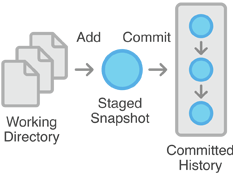
\includegraphics[scale=0.5]{imagenes/add.png}
\end{figure}
\end{frame}



\begin{frame}
\frametitle{git commit}
\begin{itemize}[<+->]
\item El comando \emph{git commit} confirma la instantánea preparada a la historia del proyecto. 
\item Las instantáneas confirmadas pueden considerarse versiones ''seguras'' de un proyecto.
\end{itemize}
\pause
\begin{verse}
git add Hello.java\\
git commit
\end{verse}
\pause
Esto abre un fichero con el editor donde podemos indicar cosas como:
\begin{verse}
Añadiendo método saludoEnIngles();\\
Añadiendo método saludoEnAleman();
\end{verse}
\end{frame}



\begin{frame}[fragile]
\frametitle{git status}
\begin{itemize}[<+->]
\item El comando git status muestra el estado del directorio de trabajo y del área de preparación. 
\item Permite ver qué cambios se han preparado, cuáles no, y qué archivos no llevan seguimiento de Git.
\item Simplemente muestra que ocurre con git add y git commit. 
\item Ejemplo:
\end{itemize}
\pause

\begin{scriptsize}
\begin{verbatim}
# Edita Hello.java
git status
# Hello.java aparece en la lista "Cambios no preparados para para confirmar"
git add Hello.java
git status
# Hello.java aparece en la lista "Cambios para ser confirmados"
git commit
git status
# nada que confirmar (directorio de trabajo limpio)
\end{verbatim}
\end{scriptsize}
\end{frame}

\begin{frame}[fragile]
\frametitle{git diff} 
Nos muestra las diferencias cuando se realiza un cambio y no es confirmado.
\begin{verbatim}
usuario@portatil:~/git$ git diff
diff --git a/Hello.java b/Hello.java
index 93e44e3..344d0aa 100644
--- a/Hello.java
+++ b/Hello.java
@@ -1,5 +1,6 @@
 public class Hello.java{
        public static void main(String[] arg){
-               System.out.println("Hola mundo");
+               System.out.println("Hola mundo");       
+               System.out.println("Hello world");      
        }
}
\end{verbatim}
\end{frame}




\begin{frame}[fragile]
\frametitle{git log}
Nos permite visualizar un histórico de las confirmaciones (\emph{commit}).
\begin{tiny}
\begin{verbatim}
commit cfd595f47194c9a0c7c2adb22c405b5b08e4f111
Author: manuel molino <push.default>
Date:   Sun Oct 19 13:58:09 2014 +0200

    tercera compilación

commit 4544fdd7e7718f5763ccf2c534a7009b21bfdd92
Author: manuel molino <push.default>
Date:   Sun Oct 19 13:53:54 2014 +0200

    segunda compilación

commit ebbf14e6963b53984d5552311cecbff6b39cf507
Author: manuel molino <push.default>
Date:   Sun Oct 19 13:53:17 2014 +0200

    primera compilación

\end{verbatim}

\end{tiny}
\end{frame}

\begin{frame}[fragile]
\frametitle{git log}
Ejecutanto el comando \emph{git log --stat --pretty}
\begin{verbatim}
commit ebbf14e6963b53984d5552311cecbff6b39cf507
Author: manuel molino <push.default>
Date:   Sun Oct 19 13:53:17 2014 +0200

    primera compilación

 Hello.java |   5 +++--
 Hola.class | Bin 0 -> 442 bytes
 Hola.java  |   6 ++++++
 3 files changed, 9 insertions(+), 2 deletions(-)

commit 98e83a8044cffcf5b66c6bc0a3e58477556db724
Author: manuel molino <push.default>
Date:   Sun Oct 19 13:43:57 2014 +0200

    Creación de fichero java

 Hello.java | 5 +++++
 1 file changed, 5 insertions(+)
\end{verbatim}
\end{frame}

\begin{frame}
\frametitle{Deshaciendo cosas}
No siempre se puede deshacer.\\
 Se usa el comando \emph{git commit - -amend}
 \pause
\begin{verse}
git commit -m initial commit\\
git add forgotten\_file \\
git commit - -amend
\end{verse}
\pause
Abré el editor y puedes cambiar el commit (\emph{initial commit})
\end{frame}

\begin{frame}[fragile]
\frametitle{Volviendo a una versión anterior}
\begin{verbatim}
$ git log
commit 7b94588...
Author: Carlos López
Date: Mon Jun 10 13:10:33 2013 +0200

<descripción de los cambios>

commit 6b1b744...
Author: Carlos López
Date: Mon Jun 10 13:00:33 2013 +0200

<estado anterior del código>
[...]
\end{verbatim}
Deshacemos con:
\begin{verbatim}
git reset --hard 6b1b744...
\end{verbatim}
\end{frame}

\begin{frame}[fragile]
\frametitle{Ejercicio}
\begin{itemize}[<+->]
\item Realiza un fork del repositorio \emph{https://github.com/manoloIESvirgendelcarmen/prueba.git}
\item Prepara un fichero \emph{.gitignore} para que no se realice un seguimiento de los ficheros \emph{.class} ni la documentación.
\item Completa el código del fichero \emph{Reapso.java} y realiza un \emph{commit}. Previamente habrás compilado la clase para saber que no tiene errores.
\item Modifica el \emph{commit} anterior como si hubieras cometido una error y quieres modificar el contenido del \emph{commit}
\item Crea la documentación del archivo \emph{Reapaso.java} usando la utilidad \emph{javadoc}, incluyendo autor y versión.
\item Genera la documentación en un directorio denominado \emph{doc}, previamente incluye dicho directorio en .gitignore y comprueba que no es añadido al repositorio.
\end{itemize}
\end{frame}


\section{GitHub}


\begin{frame}
\frametitle{Introducción a GitHub}
\begin{itemize}[<+->]
\item Es una plataforma de desarrollo colaborativo de software. 
\item Utilizado para el sistema de control de versiones Git. 
\item El código se almacena de forma pública, aunque también se puede hacer de forma privada, creando una cuenta de pago.
\item Posee una Wiki para cada proyecto.
\item Página web para cada proyecto.
\item Gráfico para ver cómo los desarrolladores trabajan en sus repositorios y bifurcaciones del proyecto.
\item Funcionalidades como si se tratase de una red social, como por ejemplo: seguidores.
\item \url{https://github.com/}
\end{itemize}
\end{frame}



\begin{frame}
\frametitle{Trabajando con repositorios remotos}
\begin{itemize}[<+->]
\item Los repositorios remotos son versiones de tu proyecto que se encuentran alojados en Internet o en algún punto de la red.
\item Puedes tener varios, cada uno de los cuales puede ser de sólo lectura, o de lectura/escritura, según los permisos que tengas.
\item Colaborar con otros implica gestionar estos repositorios remotos, y mandar (\emph{push}) y recibir \emph{(pull)} datos de ellos cuando necesites compartir cosas. 
\end{itemize}
\pause
Mostramos repositorios remotos con:
\begin{verse}
git remote -v
\end{verse}
\pause
Añadiendo repositorios remoto:
\begin{verse}
git remote add pb git://github.com/paulboone/ticgit.git
\end{verse}
\pause
Ahora puedes usar la cadena ''pb'' en la línea de comandos, en lugar de toda la URL. 
\end{frame}

\begin{frame}
\frametitle{Trabajando con repositorios remotos}
Recuperando la información de un repositorio:
\begin{verse}
git fetch pb\\
git pull
\end{verse}
\pause
Enviando a tus repositorios remotos:
\begin{verse}
git push origin master
\end{verse}
\pause
Envia la rama maestra (\emph{master}) a tu servidor origen (\emph{origin})
\pause
Inspeccionando un repositorio remoto:
\begin{verse}
git remote show origin
\end{verse}
\pause
Eliminando repositorios remotos:
\begin{verse}
git remote rm pb
\end{verse}
\pause
Renombrado repositorios remotos:
\begin{verse}
git remote rename pb paul
\end{verse}
\end{frame}

\begin{frame}[fragile]
\frametitle{Ejercicio}
\begin{itemize}[<+->]
\item Crea un repositorio denominiado \emph{Ejercicio} en tu \emph{GitHub}
\item Crea un repositorio local que nos sirva para sincronizar el repositorio antes creado.
\item Configura el fichero .gitignore para una aplicación típica de java.
\item Crea un archivo \emph{TipoDias.java} que nos pida un día de la semana y que nos diga si es un dia laboral o no. Usa un switch para ello. Realizalo en tu repositorio local y posteriormente sincronízalo con el de GitHub.
\item Ahora en gitHub añade la documentación de javadoc y posteriormente sincroniza con tu repositorio local.
\end{itemize}
\end{frame}

\begin{frame}[fragile]
\frametitle{Ejercicio}
\begin{itemize}[<+->]
\item Crea un repositorio nuevo en tu GitHub
\item Sincronízalo con el creado en el primer ejercicio.
\item Añade algún colaborador a tu repositorio.
\item Dicho compañero debe añadir a dicho repositorio una clase denominada \emph{TringuloEquilatero.java}, que contenga dos métodos, uno para calcular el perímetro del triangulo y otro el área.
\item Vuelve a sincronizar los repositorios de ambos componentes.
\item Analizar los commit del repositorio.
\end{itemize}
\end{frame}

\begin{frame}
\frametitle{Ramas}
\begin{itemize}[<+->]
\item Para entender realmente cómo ramifica Git, previamente hemos de examinar la forma en que almacena sus datos.
\item En cada confirmación de cambios (commit), Git almacena:
\begin{enumerate}
\item Un punto de control que conserva: un apuntador a la copia puntual de los contenidos preparados (staged), unos metadatos con el autor y el mensaje explicativo.
\item Uno o varios apuntadores a las confirmaciones (commit) que sean padres directos de esta (un padre en los casos de confirmación normal, y múltiples padres en los casos de estar confirmando una fusión (merge) de dos o mas ramas).
\end{enumerate} 
\item Para ilustrar esto, vamos a suponer, por ejemplo, que tienes una carpeta con tres archivos, que preparas (stage) todos ellos y los confirmas (commit). 
\end{itemize}
\pause
\begin{verse}
git add README.md test.rb LICENSE\\
git commit -m 'initial commit of my project'
\end{verse}
\end{frame}

\begin{frame}
\frametitle{Ramas}
En este momento, el repositorio de Git contendrá cinco objetos: un 'blob' para cada uno de los tres archivos, un árbol con la lista de contenidos de la carpeta y una confirmación de cambios (commit) apuntando a la raiz de ese árbol y conteniendo el resto de metadatos pertinentes:
\begin{figure}
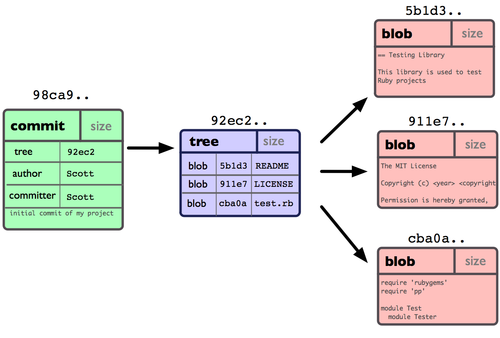
\includegraphics[scale=0.8]{imagenes/rama1.png}
\end{figure}
\end{frame}

\begin{frame}
\frametitle{Ramas}
Si haces más cambios y vuelves a confirmar, la siguiente confirmación guardará un apuntador a esta su confirmación precedente. Tras un par de confirmaciones más, el registro ha de ser algo parecido a:
\begin{figure}
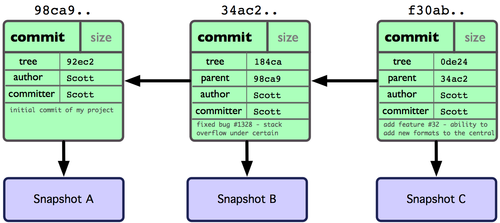
\includegraphics[scale=1]{imagenes/rama2.png}
\end{figure}
\end{frame}

\begin{frame}
\frametitle{Ramas}
Una rama Git es simplemente un apuntador móvil apuntando a una de esas confirmaciones. La rama por defecto de Git es la rama \emph{master}
\begin{figure}
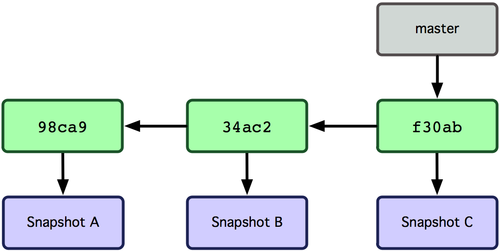
\includegraphics[scale=1]{imagenes/rama3.png}
\end{figure}
\end{frame}

\begin{frame}
\frametitle{Ramas}
Podemos crear nuevas ramas con el comando \emph{git branch nombre\_ramaNueva}\\
\pause
Ejemplo:
\begin{verse}
git branch testing
\end{verse}
\pause
Esto creará un nuevo apuntador apuntando al mismo commit donde estés actualmente:
\begin{figure}
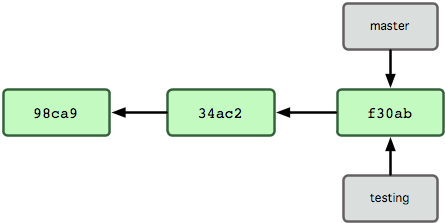
\includegraphics[scale=0.85]{imagenes/rama4.png}
\end{figure}
\end{frame}

\begin{frame}
\frametitle{Ramas}
Y, ¿cómo sabe Git en qué rama estás en este momento? Pues mediante un apuntador especial denominado \emph{HEAD}
\begin{figure}
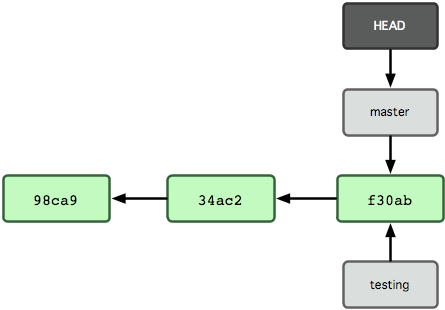
\includegraphics[scale=1]{imagenes/rama5.png}
\end{figure}
\end{frame}

\begin{frame}
\frametitle{Ramas}
Para saltar de una rama a otra tenemos el comando \emph{git checkout testing} el cuál hace:
\begin{figure}
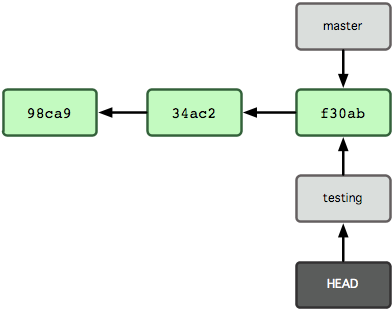
\includegraphics[scale=1]{imagenes/rama6.png}
\end{figure}
\end{frame}

\begin{frame}
\frametitle{Ramas}
¿Qué ocurre si hacemos lo siguiente?
\begin{verse}
vim test.rb\\
git commit -a -m 'made a change'
\end{verse}
\begin{figure}
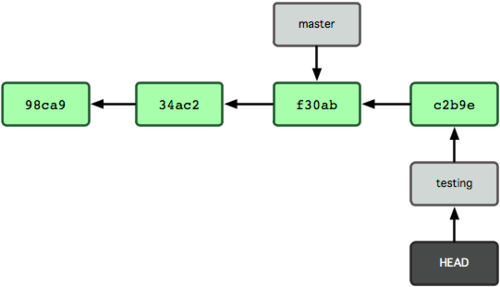
\includegraphics[scale=1]{imagenes/rama7.png}
\end{figure}
\end{frame}

\begin{frame}
\frametitle{Ramas}
¿Qué ocurre si hacemos lo siguiente?
\begin{verse}
git checkout master\\
vim test.rb\\
git commit -m 'made other change'
\end{verse}
\begin{figure}
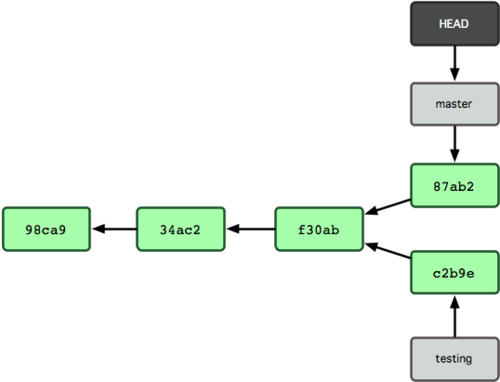
\includegraphics[scale=0.8]{imagenes/rama8.png}
\end{figure}
\end{frame}


\begin{frame}
\frametitle{Creación de ramas}
Creación de una rama y posteriormete nos posicionamos en ella:
\begin{verse}
git branch iss53\\
git checkout iss53
\end{verse}
\pause
Se pueden hacer los dos pasos a la vez:
\begin{verse}
git checkout -b iss53
\end{verse}
\begin{figure}
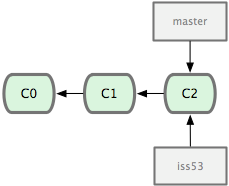
\includegraphics[scale=0.8]{imagenes/rama9.png}
\end{figure}
\end{frame}

\begin{frame}
\frametitle{Creación de ramas}
En el caso de que creemos un fichero y ejecutamos tanto el \emph{add} y el \emph{commit} quedará
\begin{figure}
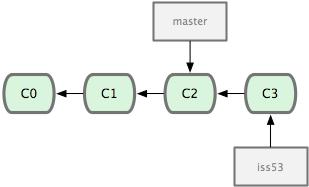
\includegraphics[scale=0.8]{imagenes/rama10.png}
\end{figure}
\end{frame}




\begin{frame}
\frametitle{Creación de ramas}
¿Qué ha ocurrido aquí?
\begin{figure}
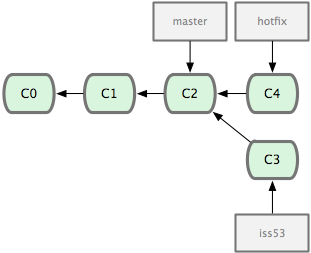
\includegraphics[scale=0.8]{imagenes/rama11.png}
\end{figure}
\end{frame}


\begin{frame}
\frametitle{Fusionando ramas}
\begin{itemize}[<+->]
\item Debemos situarnos en la rama que queremos recibir la rama a fusionar,
\item Posteriormente fusionamos.
\end{itemize}
\pause
En dos pasos, fusionando la hotfix con la master:
\begin{verse}
git checkout master\\
git merge hotfix
\end{verse}
\begin{figure}
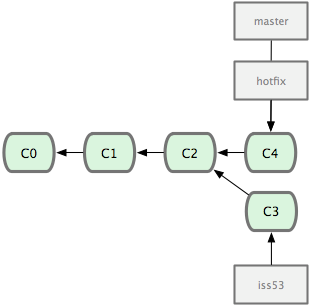
\includegraphics[scale=0.8]{imagenes/rama12.png}
\end{figure}
\end{frame}

\begin{frame}
\frametitle{Borrando ramas}
Supuesto que hemos resuelto el problema con la creación de la rama \emph{hotfix} y posteriormente fusionandola con la rama \emph{master}, es interesante borrar dicha rama con:
\pause
\begin{verse}
git branch -d hotfix
\end{verse}
\end{frame}

\begin{frame}
\frametitle{Problemas en la fusión de ramas}
\begin{itemize}[<+->]
\item En algunas ocasiones, los procesos de fusión no suelen ser fluidos. Si hay modificaciones dispares en una misma porción de un mismo archivo en las dos ramas distintas que pretendes fusionar, Git no será capaz de fusionarlas directamente. 
\item Git no crea automáticamente una nueva fusión confirmada (merge commit). Sino que hace una pausa en el proceso, esperando a que tu resuelvas el conflicto. 
\item Todo aquello que sea conflictivo y no se haya podido resolver, se marca como ''sin fusionar'' \emph{(unmerged)}
\item Git añade a los archivos conflictivos unas marcas especiales de resolución de conflictos. 
\item Estas marcas o marcadores te ayudan cuando abres los archivos implicados y los editas manualmente para corregirlos. 
\end{itemize}
\end{frame}

\begin{frame}[fragile]
\frametitle{Problemas en la fusión de ramas}

\begin{verbatim}
<<<<<<< HEAD:index.html
<div id="footer">contact : email.support@github.com</div>
=======
<div id="footer">
  please contact us at support@github.com
</div>
>>>>>>> iss53:index.h
\end{verbatim}
\pause
\begin{tiny}

\begin{verbatim}
Donde nos dice que la versión en HEAD (la rama master, la que habias activado antes de lanzar
el comando de fusión), contiene lo indicado en la parte superior del bloque 
(todo lo que está encima de =======). Y que la versión en iss53 contiene
el resto, lo indicado en la parte inferior del bloque. Para resolver
el conflicto, has de elegir manualmente contenido de uno o de otro lado.
Por ejemplo, puedes optar por cambiar el bloque, dejándolo tal que:
\end{verbatim}

\end{tiny}
\pause
\begin{verbatim}
<div id="footer">
please contact us at email.support@github.com
</div>

\end{verbatim}

\end{frame}


\begin{frame}
\frametitle{Buenas prácticas}
\begin{footnotesize}
\begin{itemize}[<+->]
\item Se deben utilizar 4 tipos de ramas: Master, Development, Features, y Hotfix.
\begin{description}
\item[Master] Es la rama principal. Contiene el repositorio que se encuentra publicado en producción, por lo que debe estar siempre estable.
\item[Development] Todas las nuevas funcionalidades se deben integrar en esta rama. Luego que se realice la integración y se corrijan los errores, se puede hacer un \emph{merge} de \emph{development} sobre la rama \emph{master}.
\item[Features] Cada nueva funcionalidad se debe realizar en una rama nueva, específica para esa funcionalidad. Estas se deben sacar de \emph{development}. Una vez que la funcionalidad esté pronta, se hace un \emph{merge} de la rama sobre \emph{development}, donde se integrará con las demás funcionalidades.
\item[Hotfix] Son bugs que surgen en producción, por lo que se deben arreglar y publicar de forma urgente. Es por ello, que son ramas sacadas de \emph{master}. Una vez corregido el error, se debe hacer un \emph{merge} de la rama sobre \emph{master}. Al final, para que no quede desactualizada, se debe realizar el \emph{merge} de \emph{master} sobre \emph{development}.
\end{description}
\end{itemize}
\end{footnotesize}
\end{frame}

\begin{frame}[fragile]
\frametitle{Ejercicio}
\begin{itemize}[<+->]
\item Crea un archivo denominado \emph{Matematicas.java} e implementa un método con la siguiente definción \emph{public static boolean esPar(int numero)}.
\item Crea un archivo \emph{TestMatematicas.java} que lea un número desde la entrada estándar y compruebe el método \emph{esPar}
\item Crea una nueva rama denominada \emph{desarrollo} donde implementes los siguientes métodos:
\begin{enumerate}
\item \emph{public static boolean esDivisiblePorTres(int numero)}
\item \emph{public sttic boolean esDivisiblePorCinco(int numero)}
\item Comprueba ambos métodos en la clase \emph{Matematicas.java}
\end{enumerate}
\item Fusiona ambas ramas y resuelve conflictos si los hubiera.
\item Borra la rama \emph{desarrollo}
\item Sincroniza el proyecto con tu \emph{gitHub}
\end{itemize}
\end{frame}


\begin{frame}
\frametitle{Preguntas} 
\begin{figure}

\includegraphics[scale=0.9]{imagenes/dudas.png} 
\end{figure} 
\end{frame}


\end{document}

